\section{ASCbase::hbond\_\-point\_\-t Class Reference}
\label{classASCbase_1_1hbond__point__t}\index{ASCbase::hbond_point_t@{ASCbase::hbond\_\-point\_\-t}}
A \char`\"{}fit\char`\"{} hbonding point.  


{\tt \#include $<$hbond\_\-points.H$>$}

Inheritance diagram for ASCbase::hbond\_\-point\_\-t::\begin{figure}[H]
\begin{center}
\leavevmode
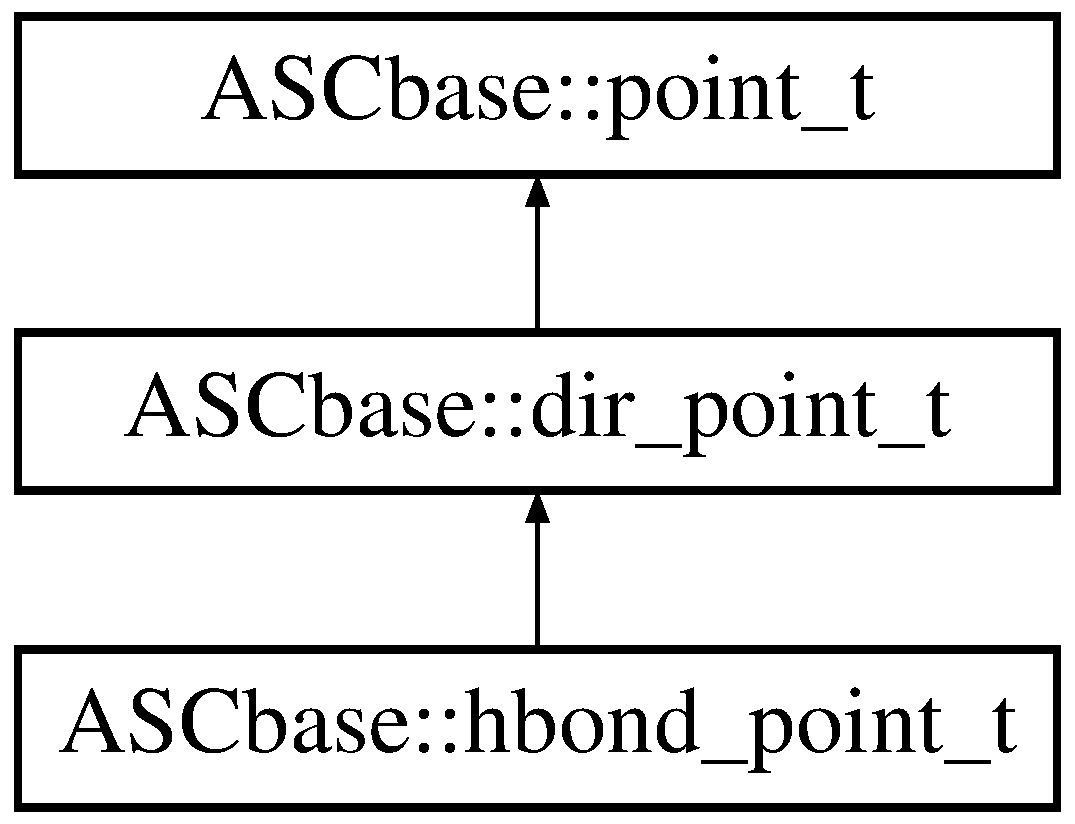
\includegraphics[height=3cm]{classASCbase_1_1hbond__point__t}
\end{center}
\end{figure}
\subsection*{Public Member Functions}
\begin{CompactItemize}
\item 
\textbf{hbond\_\-point\_\-t} (alloc\_\-t a=ALLOC\_\-POSITION)\label{classASCbase_1_1hbond__point__t_5fab75a5579f51c63612ddb147c3eb0a}

\item 
\textbf{hbond\_\-point\_\-t} (const \bf{hbond\_\-point\_\-t} \&p)\label{classASCbase_1_1hbond__point__t_a0e83b45350073eb28ceefc0c995861c}

\item 
const \bf{hbond\_\-point\_\-t} \& \textbf{operator=} (const \bf{hbond\_\-point\_\-t} \&p)\label{classASCbase_1_1hbond__point__t_c77fa3dc05e58c6cede53e560f663291}

\item 
const \bf{ASCbase::atom\_\-t} \& \textbf{\_\-\_\-get\_\-atom} () const \label{classASCbase_1_1hbond__point__t_faf40b7877ec78b4a2e134369fb5e8cf}

\item 
const \bf{ASCbase::hbond\_\-ideal\_\-point\_\-t} \& \textbf{\_\-\_\-get\_\-ideal\_\-pt} () const \label{classASCbase_1_1hbond__point__t_ed40f565437b493c187f56297417d2ec}

\end{CompactItemize}
\subsection*{Static Public Member Functions}
\begin{CompactItemize}
\item 
static bool \textbf{cmp} (const \bf{hbond\_\-point\_\-t} \&A, const \bf{hbond\_\-point\_\-t} \&B)\label{classASCbase_1_1hbond__point__t_86692805c3b0ded25d5e64a74fb8089f}

\end{CompactItemize}
\subsection*{Public Attributes}
\begin{CompactItemize}
\item 
interaction\-Type \bf{act\_\-type}\label{classASCbase_1_1hbond__point__t_64018d64558cbf939525efb893679809}

\begin{CompactList}\small\item\em Interaction type of the points. \item\end{CompactList}\item 
hbond\_\-ideal\_\-pt\_\-vci \bf{ideal\_\-pt}\label{classASCbase_1_1hbond__point__t_9ba48d24b24579d4e3a810af1fc57453}

\begin{CompactList}\small\item\em Iterator to the associated ideal point. \item\end{CompactList}\item 
atom\_\-vci \bf{atom}\label{classASCbase_1_1hbond__point__t_efd938fefea14539848e466c7f08d325}

\begin{CompactList}\small\item\em Heavy atom giving rise to the points. \item\end{CompactList}\end{CompactItemize}
\subsection*{Private Member Functions}
\begin{CompactItemize}
\item 
void \textbf{do\_\-copy} (const \bf{hbond\_\-point\_\-t} \&p)\label{classASCbase_1_1hbond__point__t_ac9aceb4f7f609deebb437ec14b8b15a}

\end{CompactItemize}


\subsection{Detailed Description}
A \char`\"{}fit\char`\"{} hbonding point. 



The documentation for this class was generated from the following file:\begin{CompactItemize}
\item 
hbond\_\-points.H\end{CompactItemize}
